%% Version 5.0, 2 January 2020
%
%%%%%%%%%%%%%%%%%%%%%%%%%%%%%%%%%%%%%%%%%%%%%%%%%%%%%%%%%%%%%%%%%%%%%%
% TemplateV5.tex --  LaTeX-based template for submissions to the 
% American Meteorological Society
%
%%%%%%%%%%%%%%%%%%%%%%%%%%%%%%%%%%%%%%%%%%%%%%%%%%%%%%%%%%%%%%%%%%%%%
% PREAMBLE
%%%%%%%%%%%%%%%%%%%%%%%%%%%%%%%%%%%%%%%%%%%%%%%%%%%%%%%%%%%%%%%%%%%%%

%% Start with one of the following:
% DOUBLE-SPACED VERSION FOR SUBMISSION TO THE AMS
\documentclass{ametsocV5}

% TWO-COLUMN JOURNAL PAGE LAYOUT---FOR AUTHOR USE ONLY
% \documentclass[twocol]{ametsocV5}


% Enter packages here. If too many math alphabets are used,
% remove unnecessary packages or define hmmax and bmmax as necessary.

%\newcommand{\hmmax}{0}
%\newcommand{\bmmax}{0}
\usepackage{amsmath,amsfonts,amssymb,bm}
\usepackage{mathptmx}%{times}
\usepackage{newtxtext}
%\usepackage{newtxmath}

\usepackage{multirow}

%%%%%%%%%%%%%%%%%%%%%%%%%%%%%%%%

%%% To be entered by author:

%% May use \\ to break lines in title:

\title{Snowfall model validation using surface observations and an optimal estimation snowfall retrieval}

%%% Enter authors' names, as you see in this example:
%%% Use \correspondingauthor{} and \thanks{Current Affiliation:...}
%%% immediately following the appropriate author.
%%%
%%% Note that the \correspondingauthor{} command is NECESSARY.
%%% The \thanks{} commands are OPTIONAL.

    %\authors{Author One\correspondingauthor{Author name, email address}
% and Author Two\thanks{Current affiliation: American Meteorological Society, 
    % Boston, Massachusetts.}}

\authors{Franziska Hellmuth\correspondingauthor{Franziska Hellmuth, franziska.hellmuth@geo.uio.no}}

%% Follow this form:
    % \affiliation{American Meteorological Society, 
    % Boston, Massachusetts}

\affiliation{Department of Geosciences, University of Oslo, Oslo, Norway}

%% If appropriate, add additional authors, different affiliations:
    %\extraauthor{Extra Author}
    %\extraaffil{Affiliation, City, State/Province, Country}

\extraauthor{Bjørg Jenny Kokkvoll Engdahl}
\extraaffil{Norwegian Meteorological Institute, Oslo, Norway, and Department of Geosciences, University of Oslo, Oslo, Norway}

%% May repeat for a additional authors/affiliations:
\extraauthor{Trude Storelvmo}
\extraaffil{Department of Geosciences, University of Oslo, Oslo, Norway}

\extraauthor{Robert O. David}
\extraaffil{Department of Geosciences, University of Oslo, Oslo, Norway}

\extraauthor{Steven J. Cooper}
\extraaffil{University of Utah, Salt Lake City, Utah}

%\extraauthor{}
%\extraaffil{}

%%%%%%%%%%%%%%%%%%%%%%%%%%%%%%%%%%%%%%%%%%%%%%%%%%%%%%%%%%%%%%%%%%%%%
% ABSTRACT
%
% Enter your abstract here
% Abstracts should not exceed 250 words in length!
%
 

\abstract{
    In the winter, orographic precipitation falls as snow in the mid to high latitudes where it causes avalanches, affects local infrastructure, or leads to flooding during the spring thaw. We present a technique to validate operational numerical weather prediction model simulations in complex terrain. The presented verification technique uses a combined DFAR and MRR retrieval approach to obtain surface snowfall accumulation and vertical profiles of snow water at the Haukelister test site, Norway. Surface and vertical snow observations are used to validate against model simulations from the Norwegian Meteorological Institute's operational forecast system and two simulations with adjusted cloud microphysics. This method can validate not only the surface snowfall accumulation but also the precipitation in the vertical.   \\ 
    Retrieved surface snowfall is validated against measurements conducted with a double-fence automated reference gauge. In comparison produces the OESR +10.9\,\% more surface snowfall than the DFAR. The predicted surface snowfall from the operational forecast model MetCoOp ensemble prediction system (MEPS) and two additional simulations with microphysical adjustments (CTRL and ICE-T) are overestimated at the surface with +41.0\,\%, +43.8\,\%, and +59.2\,\%, respectively. Simultaneously, the CTRL and ICE-T simulations underestimate the mean snow water path by -1071.4\,\% and -523.7\,\%, respectively. \\
	The study shows that we would reach false conclusions only using surface accumulation or vertical snow water content profiles. These results highlight the need to combine ground-based in-situ and vertically-profiling remote sensing instruments to identify biases in numerical weather prediction.
}

\begin{document}

%% Necessary!
\maketitle

%%%%%%%%%%%%%%%%%%%%%%%%%%%%%%%%%%%%%%%%%%%%%%%%%%%%%%%%%%%%%%%%%%%%%
% SIGNIFICANCE STATEMENT/CAPSULE SUMMARY
%%%%%%%%%%%%%%%%%%%%%%%%%%%%%%%%%%%%%%%%%%%%%%%%%%%%%%%%%%%%%%%%%%%%%
%
% If you are including an optional significance statement for a journal article or a required capsule summary for BAMS 
% (see www.ametsoc.org/ams/index.cfm/publications/authors/journal-and-bams-authors/formatting-and-manuscript-components for details), 
% please apply the necessary command as shown below:
%
% \statement
% Significance statement here.
%
% \capsule
% Capsule summary here.


%%%%%%%%%%%%%%%%%%%%%%%%%%%%%%%%%%%%%%%%%%%%%%%%%%%%%%%%%%%%%%%%%%%%%
% MAIN BODY OF PAPER
%%%%%%%%%%%%%%%%%%%%%%%%%%%%%%%%%%%%%%%%%%%%%%%%%%%%%%%%%%%%%%%%%%%%%
%

%% In all cases, if there is only one entry of this type within
%% the higher level heading, use the star form: 
%%
% \section{Section title}
% \subsection*{subsection}
% text...
% \section{Section title}

%vs

% \section{Section title}
% \subsection{subsection one}
% text...
% \subsection{subsection two}
% \section{Section title}

%%%
% \section{First primary heading}

% \subsection{First secondary heading}

% \subsubsection{First tertiary heading}

% \paragraph{First quaternary heading}




%%% Introduction %%%%%%%%%%%%%%%%%%%%%%%%%%%%%%%%%%%%%%%%%%%%%%%%%%%
\section{Introduction}
    Forecasting precipitation quantitatively is challenging, especially in complex terrain where the evaluation of forecast models is difficult due to the sparse distribution of precipitation gauges \citep{barstad_evaluation_2005}. Furthermore, coarse-resolution numerical weather prediction (NWP) models are less skillful in simulating orographic precipitation, especially over narrow topography \citep{gowan_validation_2018}. This difficulty is unfortunate, as the forecasts of avalanches, glacier mass budgets, and flash floods depend on accurate models. 
	
	NWP models with $\leq$4\,km resolution are now increasingly capable of better representation of terrain, which is critical for predicting orographic precipitation \citep{colle_59_2000, colle_1314_2005, garvert_1314_2005, schwartz_reproducing_2014}. More importantly, the higher model resolution allows for representing small-scale phenomena such as convective dynamics \citep{gowan_validation_2018}, thus enabling more accurate simulations of precipitation's magnitude and location. Improved microphysical parameterizations can influence the distribution of latent heat release, hence generating potential vorticity, which can affect storm evolution \citep{joos_influence_2012}. Sensitivity tests varying the microphysical scheme of the Consortium for small-scale Modelling model showed that storm development depended on the correct vertical placement of the precipitation inside a modeled storm \citep{joos_influence_2012}. Therefore, accurate observations of precipitation in the vertical are required to evaluate vertical model predictions.

    Accurate surface observations of precipitation are required to validate snowfall predictions from models. However, measuring precipitation, especially snow, is a well-known challenge \citep{theriault_dependence_2012,wolff_measurements_2013,colli_improved_2015}.  Winter precipitation measurements can show more than 100\,\% difference between different observing networks where the exact values depend upon regional snowfall characteristics \citep{kochendorfer_analysis_2017}. At high wind speeds, precipitation loss can be severe. Additionally, blowing surface snow can enter the gauge and artificially enhance the reported precipitation \citep{nitu_iom_2018}. A double fence automated reference (DFAR) gauge provides a more accurate estimate of snow accumulation than single fence gauges during high wind speeds \citep{wolff_derivation_2015,kochendorfer_analysis_2017}. Nevertheless, the DFAR still has an under-catch of 10\,\% at wind speeds below 9\,m\,s$^{-1}$ and 20\,\% under-catch at wind speeds between 9\,m\,s$^{-1}$ and 20\,m\,s$^{-1}$ \citep{nitu_iom_2018}. Such uncertainties must be considered when using gauge observations to evaluate model forecasts and remote sensing algorithm estimates of snowfall \citep{wolff_derivation_2015}. 
    
    Quantitative snowfall estimates from radar-based remote sensing techniques rely on deriving a snowfall rate (S) from a radar reflectivity (Z). However, studies have shown that the estimated value S depends critically upon the choice of microphysical assumptions required for the inversion \citep{kulie_utilizing_2009}. Subsequent studies incorporated scene-specific snowflake microphysical property information into the retrieval scheme to better match environmental conditions \citep{wood_microphysical_2015}. \citet{cooper_variational_2017} used in-situ observations of snowflake particle size distribution (PSD) and habit from the Multi-Angle Snow Camera (MASC) to improve radar-based estimated snowfall at Barrow, Alaska. This study exploited an optimal estimation snowfall retrieval (OESR) approach that combined radar reflectivities, in-situ microphysical property estimates, and environmental information into a common retrieval framework to provide estimates of snowfall rate. 

    
    \citet{schirle_estimation_2019} modified the \citet{cooper_variational_2017} algorithm to the instrumentation and environmental conditions at the Haukeliseter Test Site (HTS) as part of the High-Latitude Measurement of Snowfall (HiLaMS) campaign. This scheme is used in this work to estimate both surface snowfall rates and vertical profiles of snow water content (SWC).
    
    %    
    To estimate forecast uncertainty, modeling centers utilize high-resolution ensemble prediction. For example, the Meteorological Cooperation on Operational Numerical Weather Prediction (MetCoOp) produces an Ensemble Prediction (MEPS) by perturbing the initial state for the deterministic run of the  AROME-MetCoOp model \citep[AROME-Applications of Research to Operations at Mesoscale;][]{frogner_convection-permitting_2019}. 
    
    Early versions of MEPS produced too much cloud ice with its default ICE3 cloud microphysics scheme. Thus, \citet{muller_arome-metcoop:_2017} changed the ICE3 microphysics scheme to improve the representation of fog, low-level, and cirrus clouds. More recently, \citet{engdahl_improving_2020} showed that even with the improvements, the ICE3 microphysics scheme depleted supercooled liquid water too quickly and produced a surplus of snow and graupel. For this reason, \citet{engdahl_improving_2020} introduced a series of changes to the ICE3 scheme based on the parameterization development by \citet{thompson_explicit_2004,thompson_explicit_2008}. The modified microphysics include updated ice nucleation, riming/accretion parameterization, and changes to the rain class PSD \citep{engdahl_improving_2020}. Idealized 1D experiments showed that the modified scheme prolonged the existence and produced higher amounts of supercooled liquid water \citep{engdahl_improving_2020}. Many studies with adjusted microphysical schemes, such as \citet{liu_high-resolution_2011}, have validated surface precipitation forecasts to observations, but not in the vertical. \citet{liu_high-resolution_2011} show that spatial precipitation patterns at the surface are insensitive to microphysical parametrizations. The opposite is true for the vertical. A comparison of six microphysical parametrization schemes showed most parametrization schemes resemble each other in the upper troposphere but differ by a factor of three at the surface \citep{liu_high-resolution_2011}. The two-moment schemes by \citet{lin_bulk_1983,morrison_impact_2009} show the largest discrepancies to surface observations. The \citet{lin_bulk_1983} scheme (used in ICE3) shows high precipitation efficiency with low snow and cloud water but high graupel amounts. On the other hand, the \citet{morrison_impact_2009} scheme has a low graupel production, but the snow and cloud liquid water is several times larger than other simulations. 
    

    
    This study demonstrates the added value of validating snowfall in NWP models using surface and OESR vertical profiles obtained by the advanced techniques of \citet{cooper_variational_2017} and \citet{schirle_estimation_2019} during winter 2016-2017. We use DFAR snow observations, radar-based snowfall retrievals \citep{cooper_variational_2017,schirle_estimation_2019}, and high-resolution forecast data from MEPS at the Haukeliseter test site (HTS). The instrumental setup at HTS is a unique opportunity to apply the radar snowfall retrieval by \citet{schirle_estimation_2019} and verify snowfall in the operational MEPS and sensitivity simulations with adjusted cloud microphysics conducted by \citet{engdahl_effects_2020}.
    
    We structure the remainder of this paper as follows: Section \ref{sec:methodology} describes the study location, observations, and methodology. Section \ref{sec:res} describes the snowfall regimes, followed by a validation of the OESR retrieved solid surface accumulated precipitation compared to the DFAR. Next, we discuss the seasonal bias in the accumulated solid surface precipitation and the vertical snowfall distribution of the NWP model simulations (MEPS, CTRL, and ICE-T) relative to the DFAR and OESR. Finally, Section \ref{sec:conclusion} presents the conclusions.

%%%%%%%%%%%%%%%%%%%%%%%%%%%%%%%%%%%%%%%%%%%%%%%%%%%%%%%%%%%%%%%%%%%%%

%%% Methodology %%%%%%%%%%%%%%%%%%%%%%%%%%%%%%%%%%%%%%%%%%%%%%%%%%%%%
\section{Methodology}\label{sec:methodology}
	\subsection{Haukeliseter test site}
		The World Meteorological Organization (WMO) Haukeliseter test site (HTS), shown in Fig. \ref{fig:norway_map}, is situated on a mountain plateau at 991 m above sea level in Telemark County, Norway (59.81\textdegree N, 7.21\textdegree E). The Norwegian Meteorological Institute (MET Norway), operates the WMO measurement site for snow accumulation since winter 2010-2011. The HTS is shielded from passing storm systems to the west by mountain peaks that extend up to 500 m above the site. Meanwhile, winds from the east can reach the HTS almost unobstructed (see Fig \ref{fig:norway_map} b).  

		The temperature, precipitation, and wind are measured and recorded every minute at the HTS. Snowfall accounts for approximately 50\,\% of the annual precipitation at the site, and the snow depth typically reaches two to three meters in winter \citep{wolff_derivation_2015}. Therefore, to represent the measurement of the 2-m air temperature, this analysis uses the temperature from the mast at 4.5\,m. An anemometer mounted at 10\,m, typically 8\,m, above the snow surface provides the wind speed and direction. The dominant wind directions for snowfall are westerly and south-easterly, with typical wind speeds below 20\,m\,s$^{-1}$ and 12\,m\,s$^{-1}$, respectively (see Fig. \ref{fig:windrose}). At HTS, the DFAR consists of a precipitation-weighing gauge (Geonor T-200B3) encircled by a double fence to reduce any impacts of high winds and blowing snow on the precipitation measurements \citep{goodison_wmo_1998}. An overview of the instrumentation at HTS, including the DFAR and the meteorological mast, is shown in Fig. \ref{fig:norway_map}c. 

		During the HiLaMS field campaign, which took place at HTS during the 2016-2017 winter, three additional instruments, a MASC, a particle imaging package, and a micro rain radar (MRR), were installed to study snowfall (see Fig. \ref{fig:norway_map} d). In this study, the OESR algorithm uses only the MASC and MRR. The MASC (Fig. \ref{fig:norway_map} d, left) consists of three cameras, three flashes, and two near-infrared sensors pointing at a ring center. The near-infrared sensors trigger the flashes and cameras to obtain a three-dimensional image of the hydrometeor and detect the hydrometeors as they pass through the ring. Hydrometeor fall speed is determined from the time it takes to fall between the two vertically-arranged infrared sensors \citep{garrett_fall_2012}. In addition, the MASC provides estimates of the snow crystal habit, PSD, and near-surface snowfall velocity, which were used to determine the OESR assumptions (see Section \ref{sec:methodology}\ref{sec:methodology:oesr}). 
		
		Meanwhile, the MRR (Fig. \ref{fig:norway_map} d, right) operates at 24\,GHz and was used to determine particle reflectivity and Doppler velocity aloft, thus providing the vertical macrophysical structure of snow events. The radar-based OESR retrieved profiles every minute at a vertical resolution of 100\,m between 300 and 3000\,m. 


	\subsection{Snowfall regime analysis}\label{sec:methodology:snowfall_reg}
		An analysis of the 10-m wind (Fig. \ref{fig:windrose}) indicates that most snowfalls occurred in two distinct wind regimes (west and east). Furthermore, the MRR reflectivities suggested that the precipitation's vertical structure differed depending on the wind regime, with the westerly events consisting of pulses of high reflectivities (\textgreater 25\,dbZ; see Fig. \ref{fig:MRR_refl}a). In contrast, during the easterly wind regime, the vertical reflectivity structure was associated with light precipitation ($\leq$ 25\,dbZ; see Fig. \ref{fig:MRR_refl}b). Therefore, the snowfall events were separated by wind regime, namely a westerly (202.5\textdegree to 22.5\textdegree) and an easterly (22.5\textdegree to 202.5\textdegree) regime, similarly to \citet{schirle_estimation_2019}. 

		The wind regime was assigned for each minute observation when the surface temperature was less than 2\,$^{\circ}$C depending on the observed wind direction during that minute. However, to omit local topographically induced turbulence on the wind regime assignment, a given wind regime was only assigned if it lasted for more than 10 minutes. Thus, we allow wind shifts lasting less than 10 minutes to be assigned to the encompassing wind direction. Once we determined the wind regime to the minute data, the respective OESR was used to calculate the surface accumulated snowfall and the vertical SWC. Due to instrument failures, we only considered days with continuous hourly observations (24\,h) in the analysis. Furthermore, only days are used where the DFAR and OESR observed more than 0.25\,mm\,day$^{-1}$ precipitation to exclude measurement noise from the analysis.	
		
		The DFAR measurements were summed over each hour and assigned to the instantaneous 10-m wind speed and direction at the end of the hour as measured by the anemometer at HTS to make the observations and simulations comparable. Similarly, the OESR surface accumulation was summed each hour and assigned to the instantaneous wind speed and direction at the end of the hour, regardless of the wind regime used for the OESR within the hour. We discuss the two distinct precipitation regimes with their specific meteorology, MRR reflectivities (Fig. \ref{fig:MRR_refl}), and associated snowfall in Section \ref{sec:res} \ref{sec:res:snowfall_regimes}.

	\subsection{Optimal Estimation Retrieval Algorithm}\label{sec:methodology:oesr}
		\citet{schirle_estimation_2019} describe the OESR technique used to estimate the vertical profile of snow properties. Use of the flexible OESR approach allows a means to combine radar reflectivities, in-situ observations, atmospheric temperature profiles, and a priori information into a common retrieval framework to provide an estimate of snowfall properties consistent with each. The scheme retrieves an exponential PSD for each range bin of the MRR that then can be converted to SWC using particle model size-mass dimensional relationships. The SWC is then transformed into snowfall water equivalent at the surface through use of fall speed observations. 

		
		During the HiLaMS campaign, \citet{schirle_estimation_2019} explored the impact of different microphysical assumptions in the OESR on retrieved surface snowfall. They found best-case differences between total seasonal retrieved surface accumulations and HTS DFAR observations of +\,9\,\% and +\,16\,\% during easterly and westerly snowfall regimes, respectively. However, the combination of measurements that maximized retrieval performance differed for these snowfall regimes. For the relatively low-wind easterly events, best OESR results used observations of PSD and fall speed from the MASC. For the high wind and snowfall westerly wind events, near-surface turbulence and blowing snow dictated the use of a temperature-PSD relationship and fall speeds from the MRR for best results. However, the most important assumption for the first-order accuracy of any snowfall retrieval scheme is the selection of a particle model that is well-matched to scene environmental conditions \citep{cooper_variational_2017,schirle_estimation_2019}. At HTS, partially-rimed aggregates dominated the MASC images during both wind regimes (Fig. \ref{fig:snowflakes}). As such, \citet{schirle_estimation_2019} used a snow particle aggregate model developed for the CloudSat mission that produces a high reflectivity per unit mass relationship consistent with aggregates entrained in high liquid water content aloft \citep{wood_microphysical_2015}.
		
		In this work, we use these assumptions to compare surface snowfall accumulations in the OESR with DFAR measurements for a slightly different classification scheme for snowfall events than those used in the \citet{schirle_estimation_2019}. 
		
		Good agreement between retrieved and observed snowfall values at the surface suggests confidence in the retrieved SWC values aloft. At HTS, \citet{schirle_estimation_2019} showed that using a rimed aggregate particle model produced retrieved snowfall values well matched the MET Norway DFAR observations. Given that surface snowfall characteristics are dictated by snowfall processes aloft, there should be a strong physical correlation between the aggregate particles at the surface and those the MRR measures above. The OESR scheme also uses a PSD-temperature relationship that allows PSD to change with height for more accurate in-cloud retrievals of SWC \citep{wood_estimation_2011}. Current research focuses on using airplane in-situ microphysical observations to evaluate retrieved vertical profiles of snow water. Such work, however, is beyond the scope of this paper.
	



	\subsection{Operational Weather Forecast Model - MEPS}\label{sec:methodology:MEPS}
		In this study, we make use of the archived MEPS surface forecasts, the control (CTRL) run, and a version of the CTRL with the modified microphysics scheme (ICE-T) from \citet{engdahl_effects_2020}.

		MEPS is the operational ensemble forecast system used at MET Norway \citep{frogner_convection-permitting_2019}. It is based on HARMONIE-AROME (version 40h1.1), a mesoscale non-hydrostatic, convection-permitting NWP model \citep{the_metcoop_team_metcoop_2017} which, in turn, based on the model developed by Meteo-France, AROME \citep{seity_arome-france_2010,bengtsson_harmoniearome_2017}.

		HARMONIE-AROME uses the single-moment ICE3 bulk microphysics scheme \citep{caniaux_numerical_1994,pinty_mixed-phased_1998} to represent cloud microphysics. ICE3 simulates mass mixing ratios of cloud water and ice, rain, snow, and graupel \citep{cohard_comprehensive_2000, cohard_comprehensive_2000-1}.

		Within MEPS, HARMONIE-AROME runs at a horizontal resolution of 2.5\,km with 65 hybrid levels in the vertical. Fig. \ref{fig:norway_map}a shows the MEPS model domain and simulated elevation with a domain center at 63\textdegree N, 15\textdegree E. MEPS consists of ten HARMONIE-AROME ensemble members. We use the ensemble output from the MEPS archive with initialization at 00\,UTC, with three-hourly cycling for data assimilation. The control run has initial and lateral boundary conditions from the European Centre for Medium-range Weather Forecasts (ECMWF) High-Resolution forecast. The ensemble is created by giving members one through nine perturbed initial and lateral boundary conditions based on the Scaled Lagged Average Forecasting method \citep{koltzow_metcoop_2017}. In this study, we average the ensemble members (the ensemble mean) to derive the reported MEPS variables in the following figures - a detailed description of the MEPS operational setup can the interested reader find in \citet{frogner_convection-permitting_2019}. 

	 	\citet{engdahl_effects_2020} pointed out a coding error, corrected in the CTRL run, and therefore, the CTRL microphysics deviates slightly from the archived MEPS simulations. In a follow-up study, \citet{engdahl_effects_2020} ran 3D simulations with both the bug-fixed microphysics scheme, CTRL, and ICE-T, respectively, for Dec 2016 - Feb 2017. An overview of the differences between the two microphysical schemes in CTRL and ICE-T is found in Table \ref{tab:micr_changes} and \citet{engdahl_improving_2020}. The \citet{engdahl_effects_2020} model setup is as follows: The domain has the exact horizontal and vertical resolution as MEPS but is placed further to the west to provide additional spin-up time for weather systems from the west. The CTRL and ICE-T are initialized every day at 00\,UTC. The initialization uses the initial and lateral boundaries from the operational ECMWF-Integrated Forecast System but with no surface or upper air data assimilation. Therefore, clouds and precipitation are not available at the beginning of the simulation. ICE-T led to a general increase in supercooled liquid water, a shift in hydrometeor distribution from graupel to snow, and a shift in the precipitation pattern with more precipitation spilling over to the lee side of mountain barriers \citep{engdahl_effects_2020}.
		
		
		
	\subsection{Model validation}\label{sec:methodology:MEPS_vali}
		To validate the model, we use the closest grid point to HTS, which is located 0.9\,km from the site in HARMONIE-AROME and has a similar altitude of 1041\,m above sea level. Identical to \citet{engdahl_effects_2020}, we exclude the first 12 hours of each simulation and then analyze the following 24\,h to account for the model spin-up time of clouds and precipitation in MEPS, CTRL, and ICE-T. The DFAR and OESR data are compared to the same periods as the model simulations. Hence a day of interest starts at 12\,UTC and ends the next day at 12\,UTC. Finally, the total accumulated precipitation difference within an hour is calculated for the observations and the model simulations. 
		
		Additionally, the instantaneous 2-m temperature of the observations and the model had to remain below 2\,$^{\circ}$C to ensure only snowfall is present due to the OESR setup and resulting surface snowfall accumulation and SWC from the OESR. The separation into snowfall regimes takes the instantaneous 10-m wind direction from MEPS, CTRL, and ICE-T. The simulated wind speeds were then corrected to analyze the simulated surface solid accumulation and vertical precipitation by wind speed. \citet{engdahl_effects_2020} verified CTRL and ICE-T with 177 WMO stations in Norway for the three winter months simulation and found the 10-m mean error in the wind speed of approximately +0.7\,m\,s$^{-1}$. However, the complex terrain around the HTS and its representation in MEPS, CTRL, and ICE-T leads to a greater wind bias simulation (see Fig. \ref{fig:WS_correlation}). Therefore, we analyzed the simulated and observed wind speeds, and we found a simulated bias of +2.92\,m\,s$^{-1}$, +2.44\,m\,s$^{-1}$, +2.55\,m\,s$^{-1}$ for MEPS, CTRL, and ICE-T, respectively (see Fig. \ref{fig:WS_correlation}). Hence, we corrected the simulated wind speed in the postprocessing to compare the solid surface accumulation and vertical precipitation more accurately to the corresponding observed wind speeds. 
		
		
		The MEPS archive does not provide the vertical parameters to calculate the SWC profile for all ensemble members. Hence, we did not carry out a vertical validation for MEPS simulations. Instead, we validate the instantaneous amount of snowfall in the vertical from the simulations CTRL (which we assume is close to the deterministic forecast in MEPS) and ICE-T to the OESR vertical profiles of SWC.
		
		In CTRL and ICE-T, the SWCs were derived by summing the mass mixing ratios of cloud ice, snow, and graupel and then converting to g\,m$^{-3}$ (Eq. \ref{eq:swc}) by using the vertically resolved air density (Eq. \ref{eq:dens}) of MEPS as follows:
		\begin{equation}
			SWC(\sigma) = \rho(\sigma) \cdot [m_{snow}(\sigma) + m_{graupel}(\sigma) + m_{cloud ice}(\sigma)] \cdot 10^6 \qquad (g\,m^{-3})
			\label{eq:swc}
		\end{equation}
		where
		\begin{equation}
			\rho(\sigma) = \frac{p(\sigma)}{R_d \cdot T(\sigma)}, \qquad (kg\,m^{-3})
			\label{eq:dens}
		\end{equation}
		The SWC was calculated at each $\sigma$-pressure level, but for validation, the SWC is only compared to the corresponding heights of the retrieved snowfall values from the MRR. Additionally, we compare the total snow water path (SWP) from the instantaneous values of the OESR, the CTRL, and ICE-T simulations to validate the integrated ice mass from 400 m to 3000 m over HTS. Then the SWP is calculated at each hourly instantaneous output of the model and corresponding time in the OESR with Simpson's rule (Eq. \ref{eq:swp}).
		\begin{equation}
		\begin{split}
		SWP =\\
		&\quad = \int_{h = 400\,m}^{h = 3000\,m} SWC(h) dh  \\
		&\quad = \frac{h_{3000\,m} - h_{400\,m}}{3} \left[ SWC(h_{400\,m}) + SWC(h_{3000\,m}) + 4 \cdot SWC \left( \frac{h_{400\,m} + h_{3000\,m}}{2}\right) \right], \qquad (g\,m^{-2})
		\end{split}
		\label{eq:swp}
		\end{equation}
		


%%%%%%%%%%%%%%%%%%%%%%%%%%%%%%%%%%%%%%%%%%%%%%%%%%%%%%%%%%%%%%%%%%%%%

%%% Results %%%%%%%%%%%%%%%%%%%%%%%%%%%%%%%%%%%%%%%%%%%%%%%%%%%%%%%%%
\section{Results}\label{sec:res}
	\subsection{Snowfall regimes}\label{sec:res:snowfall_regimes}
		The DFAR observed the most surface snowfall accumulation during the westerly snowfall regime, which accounted for 73\,\% (146.5\,mm, see Fig. \ref{fig:sfc_WS_WD}a) of the total precipitation during the 2016-2017 winter. In this snowfall regime, 20\,\% of the precipitation occurred at wind speeds higher than 12\,m\,s$^{-1}$ and sometimes exceeding 20\,m\,s$^{-1}$ (Fig. \ref{fig:windrose}). Fig. \ref{fig:MRR_refl} demonstrates MRR reflectivities during the two distinct snowfall regimes. Westerly snowfall events consisted of intermittent periods of heavy (\textgreater 25\,dBZ) and light (\textless 15\,dBZ) snowfall with a duration of approximately 30\,min (Fig. \ref{fig:MRR_refl}a). The observed precipitation pattern is consistent with HTS being located to the lee of the higher mountains to the west (see Fig. \ref{fig:norway_map}b). Previous studies found that latent heat release on the windward slope of mountain barriers leads to pulsed precipitation on the leeward side \citep{sinclair_factors_1997,kaplan_role_2009}. 

		In contrast, the easterly snowfall regime was associated with light precipitation of 54.0\,mm (Fig. \ref{fig:sfc_WS_WD}b) and  winds of less than  12\,m\,s$^{-1}$ (Fig. \ref{fig:windrose}). The MRR reflectivities for the easterly snowfall regime were consistent with continuous moderate precipitation with values near 15-20\,dBZe (see Fig. \ref{fig:MRR_refl}b). Moderate easterly winds likely enhanced the snowfall as the low-level easterly flow impinged the mountain barrier, causing enhanced lift and orographic precipitation. Indeed, the precipitation during the easterly snowfall regime was dominated by rimed aggregates, as shown in Fig. \ref{fig:snowflakes}b. The riming is likely due to forming a low-level feeder cloud, which acted as a source of additional condensate where the snowfall gained mass by riming \citep{borys_mountaintop_2003,lowenthal_isotopic_2016}. Indeed, Fig. \ref{fig:MRR_refl}b shows an increase in reflectivity around 1000 m above the surface between 18 and 00 UTC. The increase is likely due to the precipitation growth in the low-level feeder cloud.

	\subsection{Retrieval validation}
		During the 2016-2017 winter, a difference of 10.9\,\% between retrieved (OESR) and DFAR total surface accumulations was observed (Table \ref{tab:sfc_acc}). When separating by snowfall regime, the retrieval overestimated the accumulated surface precipitation by +7.3\,\% and +20.5\,\% during the westerly and easterly snowfall regimes, respectively (see Fig. \ref{fig:sfc_WS_WD}a and Table \ref{tab:sfc_acc}). Furthermore, when comparing the OESR and DFAR snowfall rates,  a strong correlation between the measurements of R$^2$ = 0.81 and R$^2$ = 0.71 for the westerly and easterly snowfall regimes, respectively, was observed (see Fig. \ref{fig:sfc_oesr}) - indicating that the microphysical a priori selected for the OESR are well-matched for the HTS conditions. Additionally, these results largely agree with \citet{schirle_estimation_2019}, who found a +16\,\% and +9\,\% difference between OESR and DFAR observed season snowfall accumulations during westerly and easterly events. Slight differences between the studies are likely due to the minor changes in snowfall regime classification in this study.

		Notably, the difference between the retrieved and measured precipitation could be due to the under-catch of the DFAR at high wind speeds \citep{theriault_impact_2015,nitu_iom_2018,colli_adjustments_2020}. \citet{nitu_iom_2018} showed that the DFAR has an under-catchment up to 10\,\% for wind speeds below 9\,m\,s$^{-1}$. Meanwhile, they estimated that the DFAR has an under-catch of 20\,\% during wind speed between 10\,m\,s$^{-1}$ and 20\,m\,s$^{-1}$. Thus, when accounting for the influence of wind speed on the DFAR measurements, the difference between the DFAR and OESR surface accumulation becomes -6.8 \% and +9.2 \% for the westerly and easterly regimes, respectively (see Table \ref{tab:sfc_acc}). Thus, the DFAR under-catchment can explain the observed difference between the OESR and DFAR during westerly events. In contrast, during the easterly snowfall regime, accounting for potential under-catchment does not explain the difference between the OESR and DFAR. As a result, the cumulative difference between the DFAR and OESR for the easterly snowfall regime over the entire season is only 11\,mm. 

		The similarity between the retrieved surface snowfall amount from the OESR and the DFAR suggests confidence in retrieved SWC values aloft, as discusses in Section \ref{sec:methodology}\ref{sec:methodology:oesr}. In addition, these values will be used as a reference to evaluate the vertical profiles of snow water from the CTRL and ICE-T simulations, as discussed in Section \ref{sec:res}\ref{sec:res:swc}.
	
	\subsection{Validation of surface snowfall}\label{sec:res:season_sfc}
		Following the technique described in Section \ref{sec:methodology}\ref{sec:methodology:MEPS_vali}, we compare the simulated accumulated surface snowfall of MEPS, CTRL, and ICE-T to the DFAR measurements over 27 days. Comparing MEPS, CTRL, and ICE-T reveals an overestimation of +41.0\,\%, +43.8\,\%, and +59.2\,\%, respectively (Table \ref{tab:sfc_acc}). Thus, MEPS slightly outperforms the simulations with more complex and adjusted microphysics. MEPS relies on an ensemble approach that predicts precipitation events' dynamical evolution more accurately, leading to better performance \citep{frogner_convection-permitting_2019}. When comparing the simulations with advanced microphysics, the CTRL simulation outperforms ICE-T as ICE-T simulates more precipitation over HTS than the CTRL. 
		The increase in simulated surface snowfall from CTRL to ICE-T is likely related to increased snow growth, as snow remains in the atmosphere longer due to lower fall velocities than graupel, leading to a lower precipitation rate and more surface accumulation \citep{engdahl_effects_2020}. \citet{liu_high-resolution_2011} found that the \citet{lin_bulk_1983} based scheme had less condensate in the atmosphere, combined with an excess of snowfall precipitation, and suggested a high precipitation efficiency due to a high fraction of fast-falling graupel.

		
		Indeed, \citet{engdahl_improving_2020} adjusted the ICE3 scheme to increase snow and reduce graupel in ICE-T. Additionally, \citet{engdahl_improving_2020} changed the coefficients in the mass-diameter relation ($m(D) = aD^b$) and terminal fall velocity ($v(D) = cD^d (\rho_{00}/\rho_{dref})^{0.4}$) within ICE-T. All coefficients ($a, b, c, d$) are changed for snow, while only $c$ and $d$ are changed for graupel by \citet{engdahl_improving_2020}, which leads to graupel falling more slowly and snow falling slower when $D < 600\mu m$ and faster for $D > 600\mu m$. Yet, the size distribution of snow is shifted towards smaller particles, so the net fall speed of snow is reduced. 
		
		The slower fall velocity of snowfall, in turn, leads to more simulated precipitation on the lee side of the mountains compared to CTRL (see Fig. \ref{fig:sfc_WS_WD}) through an eastward displacement in the transition from snow to graupel and an overall increase in snowfall over inland Norway \citep{engdahl_effects_2020}. Indeed, when comparing the simulated accumulated surface snowfall by snowfall regime, the westerly snowfall regime events show an overestimation at the surface of +59.7\,\%, +59.3\,\%, +79.2\,\%, for MEPS, CTRL, ICE-T, respectively (see Table \ref{tab:sfc_acc}). 
		
		Meanwhile, the simulated easterly snowfall regime events show to be within the observation uncertainty of snowfall at the surface of -9.7\,\%, +1.8\,\%, +5.0\,\% for MEPS, CTRL, and ICE-T, respectively (see Table \ref{tab:sfc_acc}). Therefore, the shift in precipitation to the lee of the mountain barrier dominates the model's overestimation during westerly events. Snowfall shift is especially the case for the ICE-T simulation, which shows the most significant overestimation during the westerly snowfall regime. 

		When limiting the westerly snowfall to wind speed below 12\,m\,s$^{-1}$, the overestimation in accumulated snowfall by MEPS and ICE-T falls to +9.6\,\% and +13.3\,\%, respectively. Simultaneously, CTRL underestimates the observed accumulated snowfall by -0.2\,\%. In contrast, above 12\,m\,s$^{-1}$, the surface snowfall accumulation during the westerly snowfall regime is greatly overestimated by +510.7\,\%, +494.0\,\%, and +557.6\,\% for MEPS, CTRL, and ICE-T, respectively (see Fig. \ref{fig:sfc_WS_WD} a). Thus, the models are simulating too much snowfall at high wind speeds. Additionally, when accounting for the number of event hours simulated by the model between 12\,m\,s$^{-1}$ and 16\,m\,s$^{-1}$, the models also simulate twice as many event hours as observed by the DFAR (see Fig. \ref{fig:sfc_WS_WD}c). At wind speeds above 16\,m\,s$^{-1}$, the simulated event hours are closer to the observations. Thus, most of the surface snowfall overestimation in the simulations stems from too many events simulated between 12\,m\,s$^{-1}$ and 16\,m\,s$^{-1}$ during the westerly regime. Additionally, the snowfall amount per event hour is overestimated at wind speeds above 12\,m\,s$^{-1}$, suggesting that models simulate too much spillover when higher wind speeds are simulated (see Fig. \ref{fig:sfc_WS_WD}d). Indeed, higher cross-mountain wind speeds result increase spillover precipitation \citep{chater_atmospheric_1998,kaplan_role_2012}. Regardless of the mechanisms responsible, the overestimation in simulated surface snowfall occurs in both the models that rely on an ensemble of NWP models (here presented as the ensemble mean of MEPS) or have altered microphysical schemes (CTRL, ICE-T). 
		
		In contrast to the westerly snowfall regime, there is no clear dependence on accumulated snowfall bias at different wind speeds during the easterly snowfall regime (Fig. \ref{fig:sfc_WS_WD}b). 
		However, when looking at the simulated amount of accumulated snowfall per event hour, the simulations have a significant bias at wind speeds above 8\,m\,s$^{-1}$ (see Fig. \ref{fig:sfc_WS_WD}f). This overestimation may be associated with enhanced orographic lifting at higher wind speeds or due to fewer event hours in the simulations. However, the exact mechanism for this bias is beyond the scope of this study.

		As previously mentioned, the DFAR is prone to underestimating precipitation at high wind speed. Therefore, some of the models' overestimations may be due to this, particularly as the largest overestimations occurred at wind speeds greater than 12\,m\,s$^{-1}$ for the westerly snowfall regime. Applying an under-catch error of 10\,\% to wind speeds below 9\,m\,s$^{-1}$ and 20\,\% to wind speeds above 10\,m\,s$^{-1}$ leads to a reduction in the overestimation of snowfall by the models at the surface over all events during the study period of +23.8\,\%, +26.3\,\%, and +39.8\,\% for MEPS, CTRL, and ICE-T, respectively (see Table \ref{tab:sfc_acc}). Although accounting for the under-catchment reduces the difference between the simulated and measured surface accumulated precipitation, it does not completely explain the simulated overestimation in this study. \citet{koltzow_verification_2020} discussed how wind-induced under-catch of surface snowfall can impact the verification of precipitation forecasts in Norway. The study used MEPS forecasts and found that wind-induced under-catch of snowfall has a considerable impact on the NWP verification, especially for single fence precipitation gauges. The use of the DFAR in this study reduces the potential biases due to under-catch and substanially increases confidence in the verification results \citep{koltzow_verification_2020}. Furthermore, if the DFAR under-catch significantly biased the observations, the difference between OESR and DFAR would be more pronounced, especially at high wind speeds. 
		
		On the contrary, at wind speeds above 16\,m\,s$^{-1}$ during the westerly snowfall regime, the DFAR observed more snowfall than estimated by the OESR, suggesting that blowing snow may have artificially elevated the accumulated snowfall measured by the DFAR at these high wind speeds. Therefore, under-catchment by the DFAR is not significantly biasing the observations. Thus, the models' overestimation in simulated snowfall is an actual bias, as the models produce too much snow at higher wind speeds (see Fig. \ref{fig:sfc_WS_WD}c and d).

		The following section investigates if the snowfall's overestimation in the simulations extends into the vertical.
				

	\subsection{Validation of the vertical distribution of snowfall}\label{sec:res:swc}
		The vertical distribution of SWC, as retrieved by the MRR using the OESR, is used to validate CTRL and ICE-T to identify if the tendency for too much simulated accumulated surface precipitation corresponds to an overestimation of SWC in the vertical.

		The MRR retrieved SWC averaged during winter 2016-2017 indicates precipitation formation near cloud top and subsequent growth of hydrometeors as the precipitation falls through the cloud (see Fig. \ref{fig:vert_swc}a). At 800\,m, the mean SWC reaches its maximum of 0.13\,g\,m$^{-3}$ and then begins to decrease as the precipitation continues to fall (see Fig. \ref{fig:vert_swc}a). 
		As the retrieved SWC depends on the observed reflectivity from the MRR, which is highly dependent on the falling hydrometeors' size, the decrease in mean SWC below 800\,m is likely due to a general decrease in the precipitation size. A decrease in hydrometeor size can occur because of snow crystal sublimation. Layers of strong wind shear are often present in mountain valleys, leading to fragmentation and subsequently reduced reflectivity of precipitation \citep{ramelli_influence_2020}. Additionally, due to upstream topography, a relatively dry boundary layer can exist in the lee of mountains where falling precipitation can sublimate, reducing the observed radar reflectivity \citep[e.g.,][]{ramelli_microphysical_2020}. Although it is unclear whether the decrease in MRR reflectivity and calculated SWC is primarily due to sublimation at HTS. 
		Thus, the maximum mean SWC is assumed to correspond to the mean cloud base height. Compared to the modeled SWC, both the CTRL and ICE-T simulations also capture a decrease in SWC at $\sim$600\,m above the surface (see Fig. \ref{fig:vert_swc}a), indicating that they correctly account for the vertical evolution of hydrometeors as they fall to the surface.

		Separating the SWC by wind regime, during the westerly snowfall regime (see Fig. \ref{fig:vert_swc}b-f), the maximum in mean SWC of 0.24\,g\,m$^{-3}$ occurs in the OESR between 800\,m and 1000\,m, especially at winds between 8\,m\,s$^{-1}$ and 16\,m\,s$^{-1}$ (Fig.\ref{fig:vert_swc}d and e). During the easterly events (Fig. \ref{fig:vert_swc}g-i), the mean SWC reaches a maximum of 0.19\,g\,m$^{-3}$ between 600\,m and 1000\,m at 4\,m\,s$^{-1}$ to 8\,m\,s$^{-1}$ (see Fig. \ref{fig:vert_swc}h). Thus, the westerly events tend to produce higher maxima in mean SWCs, consistent with a moister westerly air mass and subsequent precipitation as observed by the DFAR (see Fig \ref{fig:sfc_WS_WD}a and Table \ref{tab:sfc_acc}). Furthermore, the lowering of the maximum SWC during easterly snowfall regimes suggests that the cloud base is lower during easterly events. The cloud base lowering is consistent with the topography around HTS, with higher mountains to the west. Similarly, both CTRL and ICE-T correctly represent higher SWC during the westerly snowfall regime. However, only ICE-T reproduces the lowering of the SWC maximum during the easterly snowfall regime. 
		
		Comparing the vertical profiles of SWC from the simulations to the OESR, it is clear that the simulations underestimate the maximum in SWC. Furthermore, the simulations show significantly less variability in SWC with height, indicating that they are not correctly representing the microphysical processes. In particular, the total mean SWC simulated by CTRL is almost constant with height and has a maximum value around 0.05\,g\,m$^{-3}$ but decreases below 600\,m (Fig. \ref{fig:vert_swc}a). Similarly, the total mean SWC in ICE-T increases linearly as the precipitation falls and is higher relative to the CTRL simulation. However, the seasonal mean SWC is still too low in ICE-T, with a maximum value of 0.06\,g\,m$^{-3}$ at 1200\,m (Fig. \ref{fig:vert_swc}a). Thus, in principle, the CTRL and ICE-T simulations account for the sublimation below the cloud base but produce an overestimation in surface accumulation yet an underestimation in vertical SWC. 

		The microphysical adjustments within ICE-T lead to more SWC in the column above HTS, reducing the bias than the mean SWC retrieved with the MRR. \citep{engdahl_effects_2020}. Indeed, \citet{engdahl_effects_2020} demonstrated that the ICE-T scheme simulates an increase in the vertical distribution of snow and a slight reduction in graupel relative to CTRL above the HTS. Therefore, the ICE-T scheme allows the modeled solid hydrometeors to remain in the cloud longer due to the slower fall velocity of snow than graupel, thereby increasing the SWC in the vertical. Nevertheless, ICE-T still simulates too much surface snowfall compared to the DFAR. 
		
		Furthermore, the simulated sublimation of frozen precipitation below 1200\,m is too strong compared to the OESR over HTS(see Fig. \ref{fig:vert_swc}a). However, kindly note that for the comparison between the MRR retrieved and modeled SWC, the SWC profiles are only examined to 400\,m above the HTS. Thus, an upwind grid box could advect simulated precipitation to the HTS, where the low-level SWC is higher and missed in this analysis.

		For a better comparison of SWC based on the snowfall regime, the integrated value of SWC, SWP, is used. Recall that the accumulated snowfall at the surface for wind speeds below 12\,m\,s$^{-1}$ agreed well between DFAR, CTRL, and ICE-T. However, at higher wind speeds, the simulations overestimated snowfall accumulation. The overestimation was especially observed during the westerly snowfall regime (Fig. \ref{fig:sfc_WS_WD}a). The mean SWP divided into snowfall regimes and wind speeds could indicate if the vertical bias is similar for snowfall. In contrast to the surface accumulation, the simulated instantaneous SWP, averaged over the 27 days, is significantly underestimated relative to the OESR, which was in good agreement with the DFAR for surface snowfall (+10.9\,\% and see Fig. \ref{fig:sfc_oesr}). When analyzing the average simulated versus retrieved SWP averaged over all event hours, the CTRL and ICE-T have a deficit of 1071.4\,\% and 523.7\,\%, respectively. Separating the SWP by snowfall regimes reveals too little SWP irrespective of the snowfall regime (see Fig. \ref{fig:swp_WS_WD}). Comparing the SWP between CTRL and ICE-T, the ICE-T scheme reduced the deficit by a factor of two (1.96 for west and 2.08 for east). However, the underestimation in SWP was not consistent at all 10-m wind speeds. Specifically, during the westerly snowfall regime, the OESR observed more SWP at wind speeds below 16\,m\,s$^{-1}$, while the simulations overestimated SWP at higher wind speeds. The microphysical adjustments reduced the error in SWP in the westerly regime from -55.9\,\% (CTRL) to -40.1\,\% in ICE-T, below 16\,m\,s$^{-1}$ (see Fig. \ref{fig:swp_WS_WD}a). At westerly wind speeds higher than 16\,m\,s$^{-1}$, both simulations show an overestimation above +300\,\% in SWP mean, mainly because the MRR-retrieved SWP was close to zero at wind speeds higher than 16\,m\,s$^{-1}$. The overestimation of mean SWP at high wind speeds in CTRL and ICE-T is similar to the surface precipitation accumulation comparison. Still, it occurs at 16\,m\,s$^{-1}$ instead of 12\,m\,s$^{-1}$ during the westerly snowfall regime. During the easterly snowfall regime, there was no clear transition of underestimating SWP based on wind speed. Nevertheless, the models simulated more SWP at wind speeds above 8\,m\,s$^{-1}$. As the simulated surface accumulated snowfall and SWP show similar biases based on wind speed, we suggest that it may be due to the same reason - too high wind speeds and subsequent spillover estimated in MEPS and its counterparts (CTRL and ICE-T) \citep{muller_arome-metcoop:_2017,frogner_convection-permitting_2019}. 

		Regardless, the simulations overestimated the surface snowfall accumulation when comparing all event hours while significantly underestimating the SWP. The underestimation may be due to several factors, including a poor representation of the terrain in the model, an overzealous conversion of liquid to ice, and subsequent snow growth in the microphysics schemes. Indeed, the simulated location of the HTS was 51 meters higher and closer to the barrier crest in the model domain. Thus, the modeled precipitation would be susceptible to more spillover precipitation at high wind speeds, as was observed. Additionally, with its slower conversion of snow to graupel, ICE-T led to an increase in SWC and SWP over HTS. Therefore, it represented the vertical distribution of snowfall more accurately relative to the OESR. ICE-T gives more snowfall than the CTRL in the atmosphere and at the surface. Snow can stay longer in the atmosphere because of its lower fall velocity. Still, at the same time, the hydrometeors in ICE-T can have more mass but a lower diameter leading to more snow accumulation at the surface.  

		Nevertheless, an in-depth analysis of why these biases occur is required to improve regional models, especially in the vertical. We want to point out that this study only investigates the effects of changes to the ICE3 cloud microphysical scheme in the operational forecast model and the DFAR and MRR retrieval approach to validate forecast models. We are aware that differences between the model simulations and OESR could also be due to other aspects of the model, such as kinematic and thermodynamic structures. MET Norway continuously validates the operational model with radiosondes within the model domain. \citet{engdahl_effects_2020} showed a good agreement between modeled and observed temperature in the vertical for a drizzle test case. 
		
		Furthermore, there exists a broader range of microphysical schemes which have their advantages. For example, the one-moment microphysical scheme calculates the particle mass explicitly and diagnoses the number concentration based on the particle mass. While two-moment schemes, like ICE-T, calculate the number concentration explicitly for some hydrometeors. Higher-order schemes like the bin and three-moment scheme calculate the number concentration explicitly within bins of size intervals or simulate radar reflectivities. While the bin and three-moment schemes seem more applicable in this study, they are also more computationally expensive to run operationally \citep{morrison_impact_2009}. 

		Combining the surface and vertical validation presented in this study provides a new technique for validating operational forecast models with point measurements. For example, one might assume that microphysical adjustments should reduce the model's surface precipitation amount at high wind speeds without the vertical information However, corrections based on the surface observations alone would likely lead to further underestimating the vertical SWC, leading to other errors in simulated parameters. Thus, using both vertical and surface observations during future model development should help when adjusting microphysics schemes. 
		

%%%%%%%%%%%%%%%%%%%%%%%%%%%%%%%%%%%%%%%%%%%%%%%%%%%%%%%%%%%%%%%%%%%%%

%%% Conclusion %%%%%%%%%%%%%%%%%%%%%%%%%%%%%%%%%%%%%%%%%%%%%%%%%%%%%%
\section{Conclusion}\label{sec:conclusion}
	Here we present a new method for validating NWP model simulations in complex terrain with state-of-the-art observations. Specifically, we investigated how the model simulations from MET Norway's ensemble forecast product MEPS and two additional simulations with modified cloud microphysics schemes (CTRL and ICE-T) compared to observations and retrieved values. This study evaluated the model performance for 27 precipitation days by comparing simulated accumulated snowfall, SWC, and SWP to measurements at the HTS in Southern Norway. 

	An OESR algorithm, based on reflectivity profiles from an MRR and a priori assumptions that included ice crystal habit information provided by a MASC, was used to obtain vertical profiles of the SWC and SWP over the HTS \citep{schirle_estimation_2019}. The retrieved surface snowfall accumulation was compared to snowfall measurements from the HTS DFAR gauge to validate the OESR. The validation was conducted for two distinct snowfall regimes, where different a priori assumptions were used in the OESR, according to the estimates made by \citet{schirle_estimation_2019}. Once shown to compare well with the DFAR surface accumulation, the OESR retrieved SWC and SWP served as a reference to evaluate the vertical profiles of simulated SWC and SWP in the CTRL and ICE-T simulations.

	We found that MEPS, CTRL, and ICE-T overestimated the surface snowfall accumulation by validating model simulations with differing microphysical schemes compared to the DFAR during winter 2016-2017. The adjustments by \citet{engdahl_effects_2020} in the ICE-T scheme increased the overestimation of snowfall at the surface from 41.0\,\% (MEPS) to 59.2\,\% relative to the DFAR gauge. Additionally, we find that the overestimation is more pronounced during the westerly snowfall regime (MEPS: 59.7\,\%, CTRL: 59.3\,\%, ICE-T: 79.2\,\%). The significant overestimation of snowfall at the surface is related to the increase in simulated snow in the region of HTS, as discussed by \citet{engdahl_effects_2020}. The under-catchment of the DFAR can partially explain the overestimation of surface accumulation at 10-m wind speeds higher than 10\,m\,s$^{-1}$. However, under-catchment alone was not able to resolve the overestimation of snowfall at the surface. Furthermore, MEPS, CTRL, and ICE-T simulated more high wind speed event hours than observed. This likely contributed to the seasonal overestimation in the simulations due to more spillover precipitation reaching HTS than observed.

	In contrast, the model simulations produced too little snowfall throughout the vertical column relative to the OESR retrievals. The vertical representation of SWC in ICE-T improved relative to CTRL, likely due to the microphysical adjustments that maintained supercooled liquid water longer in the column \citep{engdahl_effects_2020}. This adjustment reduced the mean SWP bias by a factor of two from CTRL (-1071.4\,\%) to ICE-T (-523.7\,\%). 
	Nevertheless, too little snowfall in the vertical in CTRL and ICE-T is likely related to the generation of hydrometeors which are too large in the model simulations. 
	These larger and heavier hydrometeors fall out too quickly ultimately, reducing the SWC while generating too much snow at the surface.	

	As shown here, comparisons of vertical profile estimates of snow water derived from a combined DFAR and MRR retrieval approach can identify potential biases in snow water production within MEPS, CTRL, and ICE-T. However, using either surface accumulation values or vertical SWC profiles would lead to misleading conclusions regarding potential biases in snowfall production in the studied simulations at HTS. Therefore, we recommend that future model validation studies combine ground-based in-situ and vertically-profiling remote sensing instruments, where possible. In addition, we recommend the continued pursuit of event and site-specific observations of particle habit and fall speed to improve radar-based OESRs for locations with differing meteorological influences to contextualize our proposed explanations for the model biases in MEPS, CTRL, and ICE-T. Furthermore, liquid water path estimates from microwave radiometers and advanced lidar would help develop additional tools for validating NWP models' ability to predict the vertical distribution of microphysical processes correctly. 
	
	Finally, this study shows that the combination of radar and surface precipitation measurements provides the necessary information about the vertical evolution of precipitation to inform future improvements in microphysical schemes in NWP models. 


%%%%%%%%%%%%%%%%%%%%%%%%%%%%%%%%%%%%%%%%%%%%%%%%%%%%%%%%%%%%%%%%%%%%%

%%%%%%%%%%%%%%%%%%%%%%%%%%%%%%%%%%%%%%%%%%%%%%%%%%%%%%%%%%%%%%%%%%%%%
% DATA AVAILABILITY STATEMENT
%%%%%%%%%%%%%%%%%%%%%%%%%%%%%%%%%%%%%%%%%%%%%%%%%%%%%%%%%%%%%%%%%%%%%
% The data availability statement is where authors should describe how the data underlying the findings within the article can be accessed and reused. 
% Authors should attempt to provide unrestricted access to all data and materials underlying reported findings. If data access is restricted, 
% authors must mention this in the statement.
%
\datastatement
Historical real time observations can be accessed from the eklima Met Norway interface.
Three month simulations by \citet{engdahl_effects_2020} can be found at \url{https://thredds.met.no/thredds/catalog/metusers/bjorgjke-3mnd_ws/catalog.html} and archived MEPS via \url{https://thredds.met.no/thredds/catalog/meps25epsarchive/catalog.html}. The interested reader can contact the authors directly for the MRR reflectivity, OESR surface snowfall and SWC from the HiLaMS campaign. 

%%%%%%%%%%%%%%%%%%%%%%%%%%%%%%%%%%%%%%%%%%%%%%%%%%%%%%%%%%%%%%%%%%%%%
% ACKNOWLEDGMENTS
%%%%%%%%%%%%%%%%%%%%%%%%%%%%%%%%%%%%%%%%%%%%%%%%%%%%%%%%%%%%%%%%%%%%%
%
\acknowledgments
% Start acknowledgments here.
We want to thank Richard Moore from MET Norway for initiating this study. BJKE work is part of the WISLINE project funded by the Norwegian Research Council, grant 244106/E10. FH, TS, and ROD would also like to acknowledge support from the European Research Council (ERC) through Grant StG 758005. Furthermore, SJC work is part of the HiLaMS project funded by the National Science Foundation, grant \#1531690. 





%%%%%%%%%%%%%%%%%%%%%%%%%%%%%%%%%%%%%%%%%%%%%%%%%%%%%%%%%%%%%%%%%%%%%
% APPENDIXES
%%%%%%%%%%%%%%%%%%%%%%%%%%%%%%%%%%%%%%%%%%%%%%%%%%%%%%%%%%%%%%%%%%%%%
%
% Use \appendix if there is only one appendix.
%\appendix

% Use \appendix[A], \appendix[B], if you have multiple appendixes.
%\appendix[A]

%% Appendix title is necessary! For appendix title:
%\appendixtitle{}

%%% Appendix section numbering (note, skip \section and begin with \subsection)
% \subsection{First primary heading}

% \subsubsection{First secondary heading}

% \paragraph{First tertiary heading}

%% Important!
%\appendcaption{<appendix letter and number>}{<caption>} 
%must be used for figures and tables in appendixes, e.g.,
%
%\begin{figure}
%\noindent\includegraphics[width=19pc,angle=0]{figure01.pdf}\\
%\appendcaption{A1}{Caption here.}
%\end{figure}
%
% All appendix figures/tables should be placed in order AFTER the main figures/tables, i.e., tables, appendix tables, figures, appendix figures.
%
%%%%%%%%%%%%%%%%%%%%%%%%%%%%%%%%%%%%%%%%%%%%%%%%%%%%%%%%%%%%%%%%%%%%%
% REFERENCES
%%%%%%%%%%%%%%%%%%%%%%%%%%%%%%%%%%%%%%%%%%%%%%%%%%%%%%%%%%%%%%%%%%%%%
% Make your BibTeX bibliography by using these commands:
\bibliographystyle{ametsoc2014}
\bibliography{references}

%%%%%%%%%%%%%%%%%%%%%%%%%%%%%%%%%%%%%%%%%%%%%%%%%%%%%%%%%%%%%%%%%%%%%
% TABLES
%%%%%%%%%%%%%%%%%%%%%%%%%%%%%%%%%%%%%%%%%%%%%%%%%%%%%%%%%%%%%%%%%%%%%
%% Enter tables at the end of the document, before figures.
%%
%
% \textcolor{red}{
\begin{table}[t]
	\caption{List of microphysical processes which are altered in CTRL and ICE-T. Table taken from \cite{engdahl_improving_2020}.}
	\label{tab:micr_changes}
	\begin{center}
		\begin{tabular}{p{0.1\textwidth}||p{0.25\textwidth}|p{0.25\textwidth}|p{0.25\textwidth}} \hline\hline
			Experiment & Process altered               & Previous     & New \\ \hline \hline
			CTRL       & Heterogeneous ice nucleation  & Code mistake & Bugfix \\\hline
			ICE-T      & Autoconversion (cloud to rain)&\citet{khairoutdinov_new_2000} &\citet{berry_analysis_1974}\\
			& Rain accreting cloud water      & Variable efficiency \citep{muller_arome-metcoop:_2017}   & Variable efficiency (Thompson) \\
			& Heterogeneous ice nucleation    & \citet{meyers_new_1992}          & \citet{cooper_ice_1986} \\
			& Freezing of water drops        & None                         & \citet{bigg_supercooling_1953} \\
			& \multirow{2}{*}{Graupel collecting cloud water} & dry growth: \citet{ferrier_double-moment_1994}; & \multirow{2}{*}{\citet{cober_measurements_1993}} \\
			&                                                  & wet growth: \citet{musil_computer_1970} and \citet{nelson_influence_1983} &\\
			& Snow collecting cloud water     & \citet{farley_numerical_1989} & \citet{wang_collision_2000} \\
			& Rain collecting snow/graupel    & \citet{ferrier_double-moment_1994}; Eff = 1.0 & New variable: collection efficiency \\
			& Hydrometeor properties         & \citet{locatelli_fall_1974} & \citet{thompson_explicit_2008} \\
			& Rain inverse exponential Y-intercept parameter & $8x10^{6}\, m^{-4}$ (Marshal-Palmer) & Variable intercept parameter \citep{thompson_explicit_2004} \\ \hline
			
			
		\end{tabular}
	\end{center}
\end{table}
% }

\begin{table}[t]
	\caption{
		Surface snowfall accumulations for 27 precipitation days during winter 2016-2017. Separated into westerly and easterly snowfall regimes as described in Section \ref{sec:methodology}\ref{sec:methodology:snowfall_reg}. Diff defines the percentage difference in cumulative snowfall accumulation between OESR, MEPS, CTRL, ICE-T and the DFAR.\\
		The last five rows represent the adjustment to DFAR under-catch depending on the wind speed, where 10\,\% under-catch has been applied to winds below 10\,m\,s$^{-1}$ and 20\,\% under-catch for winds above 10\,m\,s$^{-1}$.
	}
	\label{tab:sfc_acc}
	\begin{center}
		\begin{tabular}{c||c|c|c|c|c|c}\hline\hline
			& West & Diff & East & Diff & Total & Diff  \\
			& (mm) & (\%) & (mm) & (\%) & (mm)  & (\%)   \\\hline\hline
			DFAR & 146.5 & & 54.0 & & 200.5 & \\\hline
			OESR & 157.2 & +7.3 & 65.1 & +20.5 & 222.3 & +10.9  \\\hline
			MEPS & 233.9 & +59.7 & 48.8 & -9.7 & 282.7 & +41.0  \\\hline
			CTRL & 233.3 & +59.3 & 55.0 & +1.8 & 288.3 & +43.8  \\\hline
			ICE-T & 262.4 & +79.2 & 56.7 & +5.0 & 319.2 & +59.2  \\\hline\hline
			DFAR & 168.7 & & 59.6 & & 228.3 & \\\hline
			OESR & 157.2 & -6.8 & 65.1 & +9.2 & 222.3 & -2.63  \\\hline
			MEPS & 233.9 & +38.6 & 48.8 & -18.1 & 282.7 & +23.8  \\\hline
			CTRL & 233.3 & +38.3 & 55.0 & -7.7 & 288.3 & +26.3  \\\hline
			ICE-T & 262.4 & +55.6 & 56.7 & -4.8 & 319.2 & +39.8  \\\hline 
			
		\end{tabular}
	\end{center}
\end{table}




%%%%%%%%%%%%%%%%%%%%%%%%%%%%%%%%%%%%%%%%%%%%%%%%%%%%%%%%%%%%%%%%%%%%%
% FIGURES
%%%%%%%%%%%%%%%%%%%%%%%%%%%%%%%%%%%%%%%%%%%%%%%%%%%%%%%%%%%%%%%%%%%%%
%% Enter figures at the end of the document, after tables.
%%



\begin{figure}[t]
	\noindent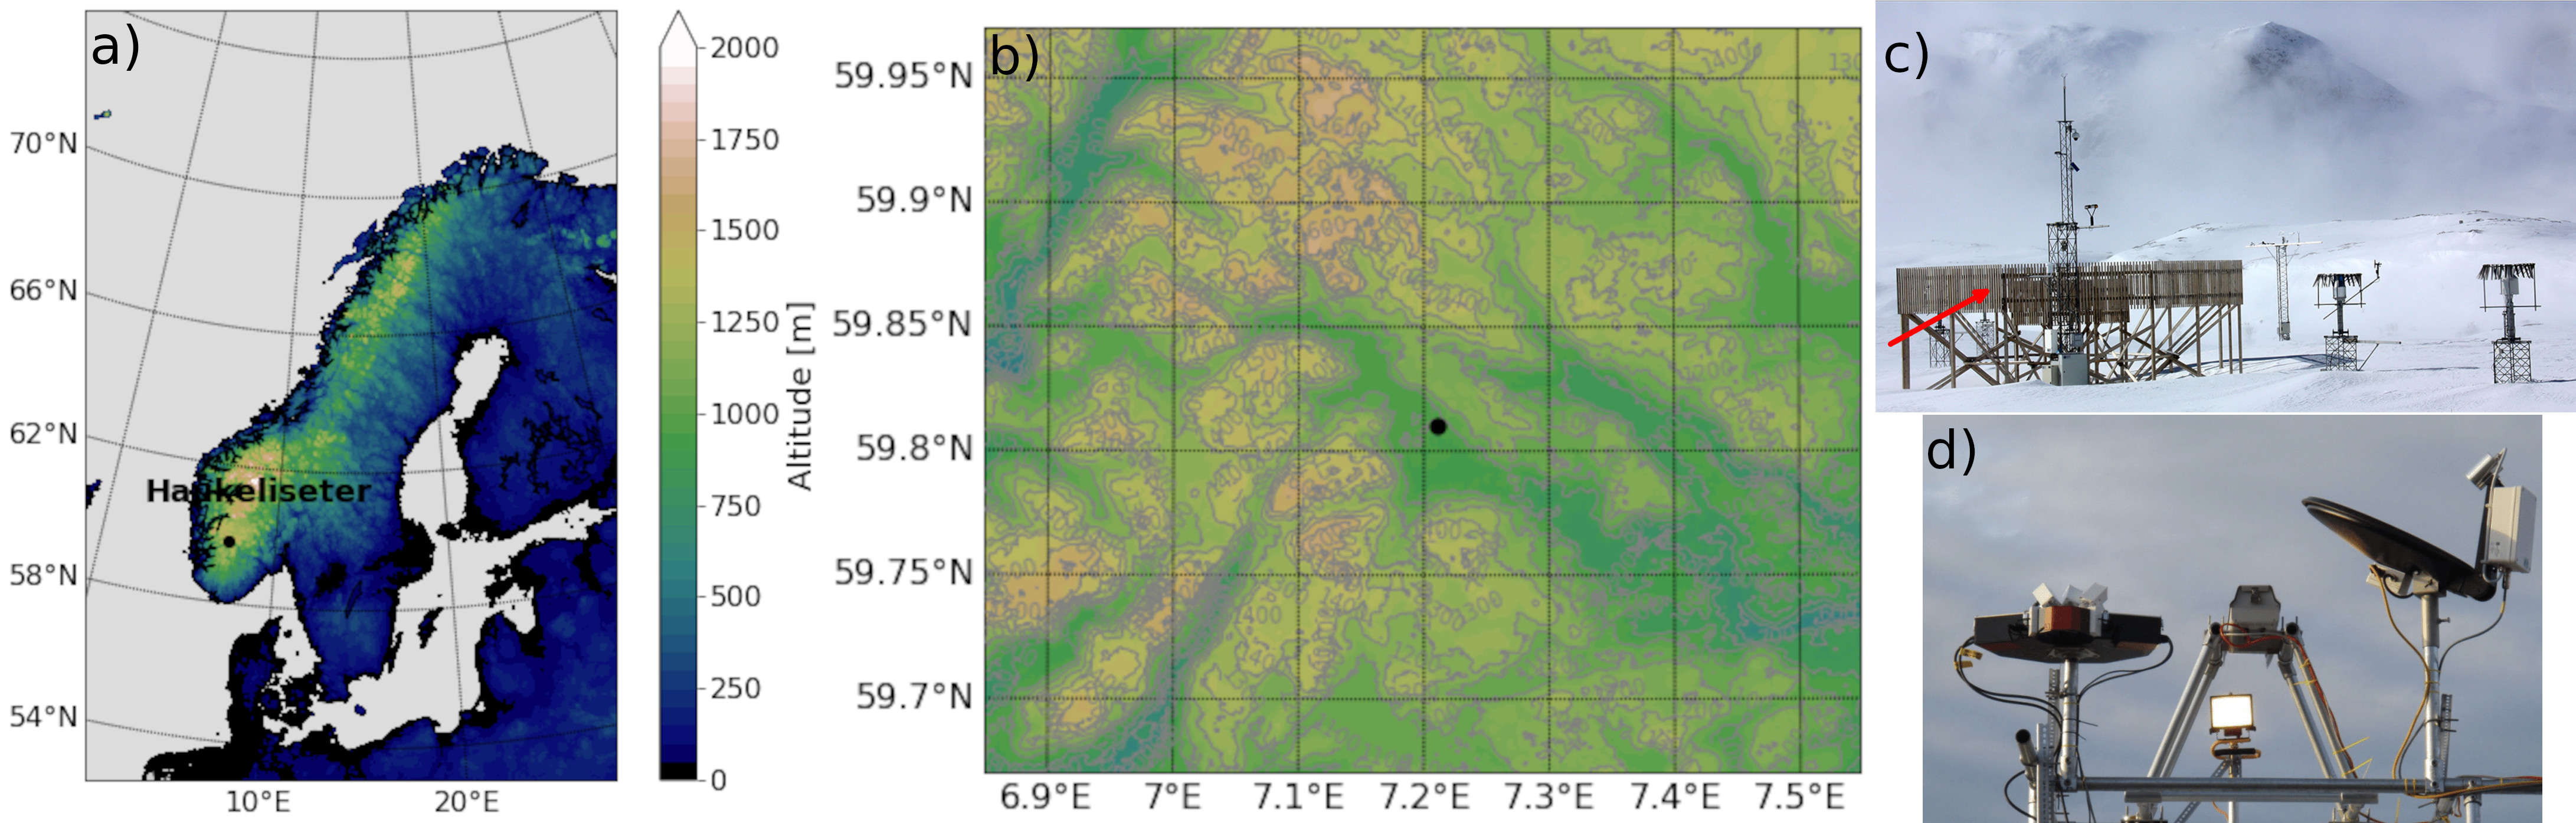
\includegraphics[width=\textwidth,angle=0]{fig1.jpg}\\
	\caption{
		a) Representation of the topography in MEPS and the MEPS model domain. HTS is located in the mountainous region in Southern Norway. The contours and shading present the elevation of the 2.5x2.5\,km grid cells. b) Topographic map around HTS. From the DTM 10 terrain model of \protect\citet{geonorge_dtm_2018}. HTS surrounded by 500\,m higher mountains to the west and more open to the south-east. \\ 
		c) DFAR, unprotected precipitation gauges and meteorological mast at HTS. The arrow indicates the westerly wind direction. The figure is adapted from \protect\citet{wolff_derivation_2015}. d) Additional instruments installed during HiLaMS during winter 2016-2017: Muli-Angle Snowflake Camera (MASC, left), Precipitation Imaging Package (middle), Micro Rain Radar (MRR, right).
	}
	\label{fig:norway_map}
\end{figure}


\begin{figure}[t]
	\noindent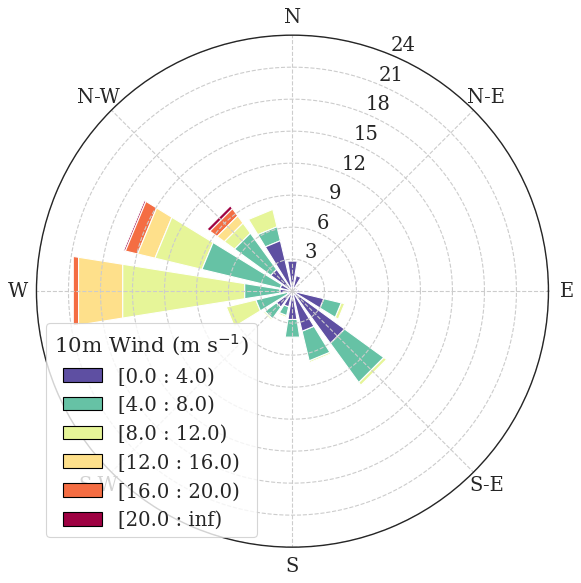
\includegraphics[width=19pc,angle=0]{fig2.png}\\
	\caption{Windrose of the 10-m wind during snowfall events when 24h accumulation $\geq$ 25\,mm\,d$^{-1}$ and 2-m temperature \textless 2\,$^{\circ}$C measured at HTS, during winter 2016-2017. Colors indicate the 10-m wind speed categories used in this study. 
	}
	\label{fig:windrose}
\end{figure}


\begin{figure}[t]
	\noindent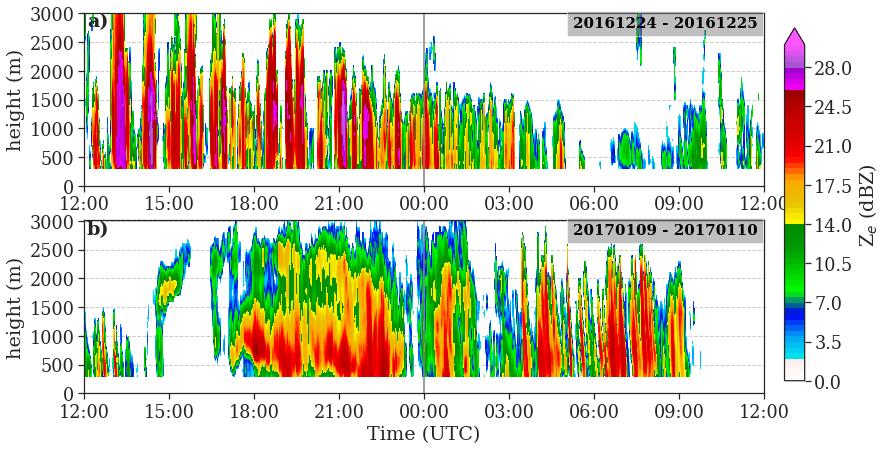
\includegraphics[width=\textwidth,angle=0]{fig4.png}\\
	\caption{Examples of MRR reflectivity during the two typical snowfall regimes. The time series for a westerly snowfall regime case during high wind speed on Dec 24-25 2016 (a). The westerly snowfall regime was associated with interchanging patterns of high and low reflectivities during snowfall. b) example during an easterly snowfall regime with low wind speeds and light precipitation of convective nature, on Jan 09-10 2017.
	}
	\label{fig:MRR_refl}
\end{figure}

\begin{figure}
	\noindent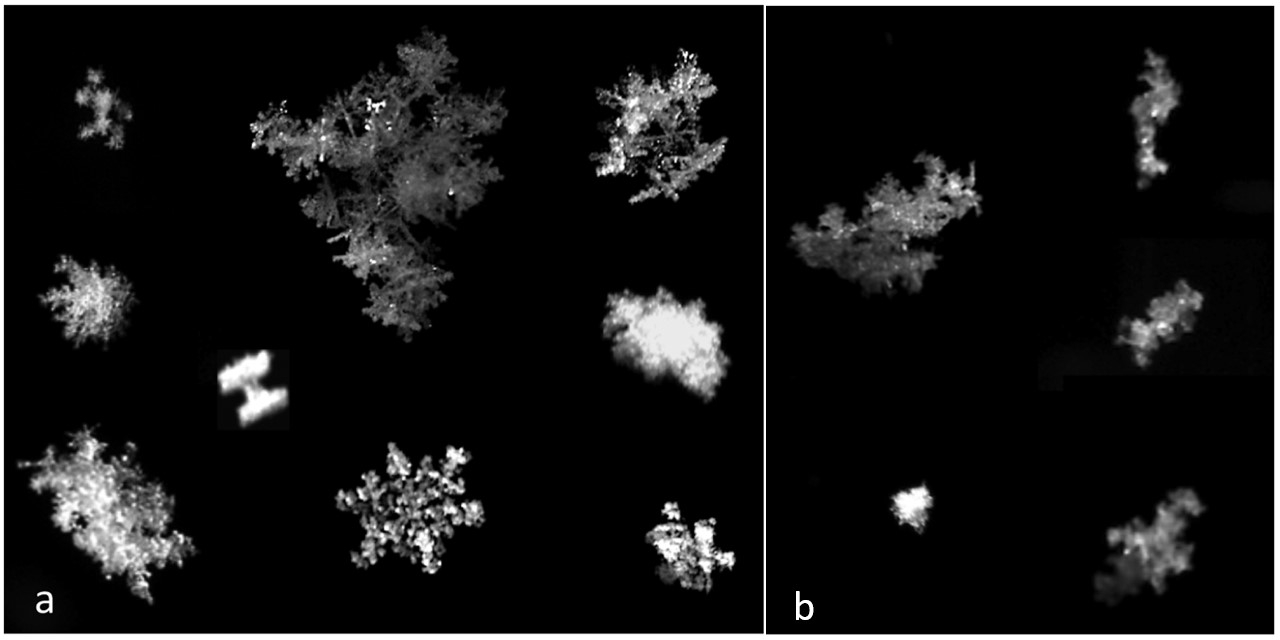
\includegraphics[width=\textwidth,angle=0]{fig5.jpg}\\
	\caption{a) Typical snowflake habits observed during events classified in the easterly snowfall regime. b) Examples of large precipitating crystals observed during the westerly snowfall regime. This figure is adapted from \protect\citet{schirle_estimation_2019}.
	}
	\label{fig:snowflakes}
\end{figure}

\begin{figure}
	\noindent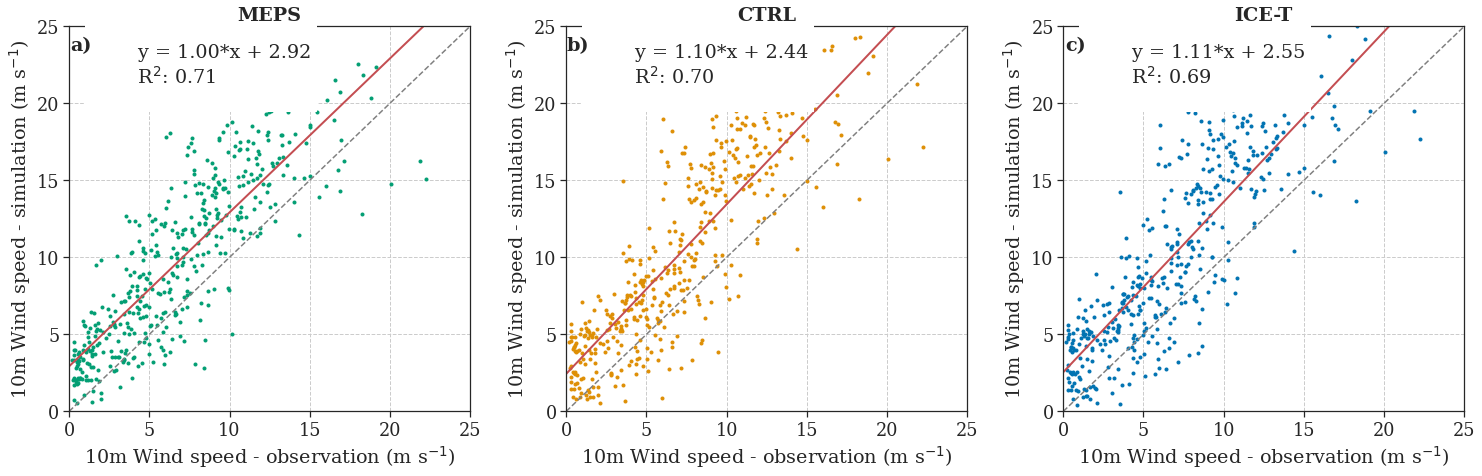
\includegraphics[width=\textwidth,angle=0]{fig6.png}\\
	\caption{Known 10-m wind bias \citep{frogner_convection-permitting_2019} was reduced according to the correlation equation between 10-m wind speeds observed at the DFAR and MEPS, CTRL, and ICE-T in a, b, and c, respectively. The red line indicates the linear correlation between DFAR and OESR. The grey dashed lines represent the line of equality where model simulations are equal to observations. 
	}
	\label{fig:WS_correlation}
\end{figure}

\begin{figure}
	\noindent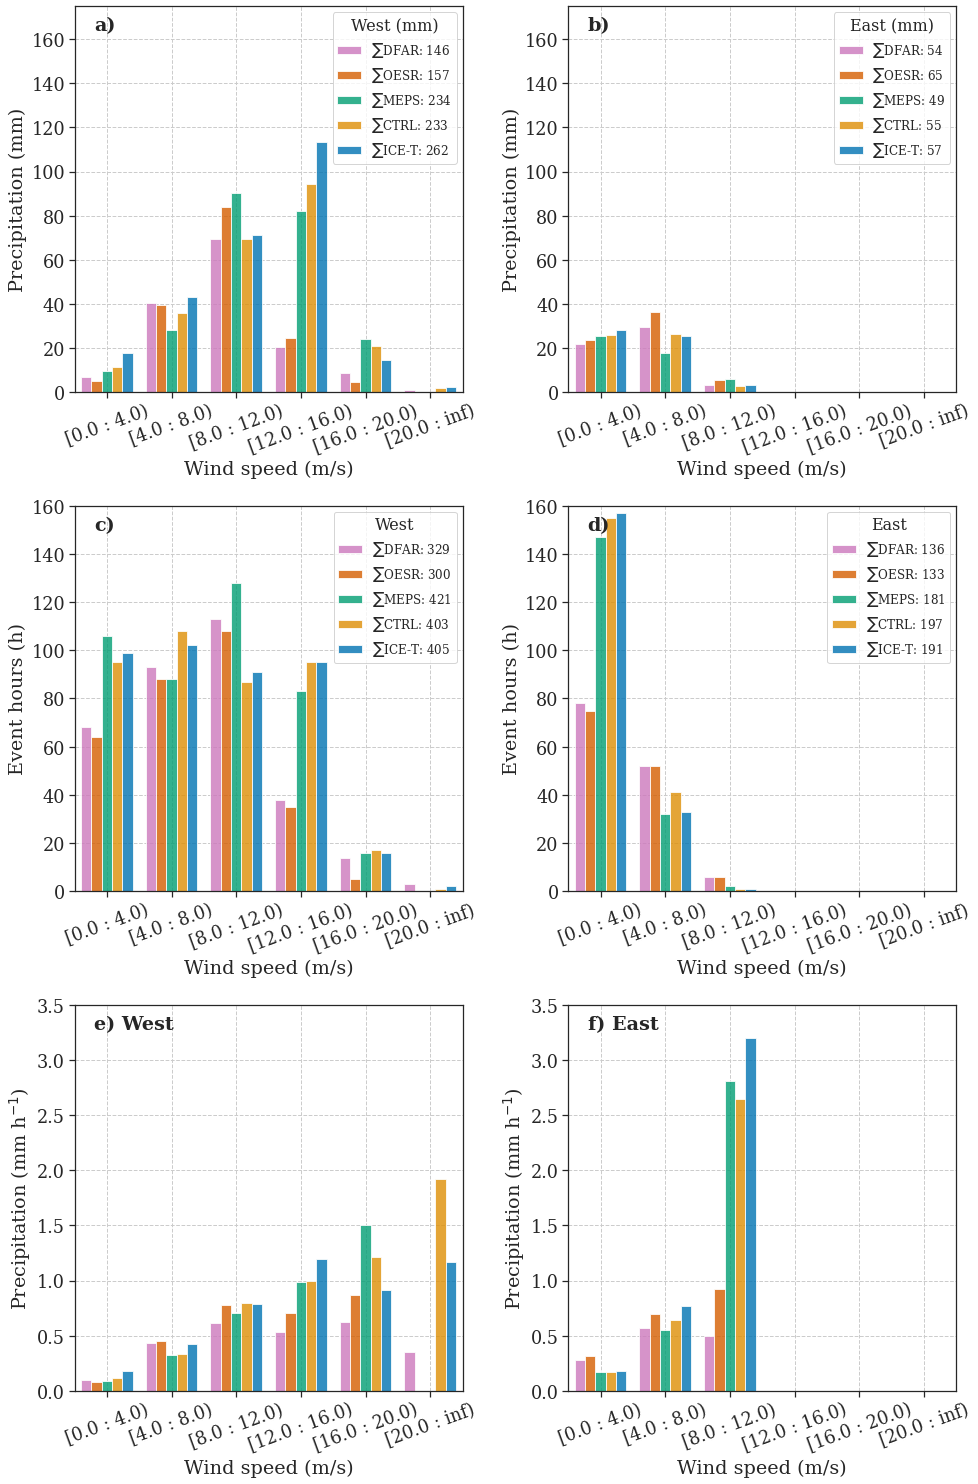
\includegraphics[width=0.65\textwidth,angle=0]{fig7.png}\\
	\caption{Surface snowfall accumulation for DFAR observations, OESR, MEPS, CTRL, and ICE-T separated into westerly (a) and easterly (b) snowfall regimes for 27 precipitation days during winter 2016-2017. The sum ($\sum$) over the 27 days of total precipitation accumulation in each snowfall regime is presented in the figure legend in a) and b). The separation into wind speed regimes is done for the corrected simulated wind according to the correlation equation in Fig. \ref{fig:WS_correlation} for MEPS, CTRL, and ICE-T. c) and d) show the event hours observed at the DFAR and OESR as well as the simulated precipitation hours in the NWPs. The total sum ($\sum$) of the precipitation hours is presented in the figure label for the 27 precipitation days. Further, the snowfall accumulation is divided by the event hours in e) and f) for westerly and easterly, respectively.
	}
	\label{fig:sfc_WS_WD}
\end{figure}

\begin{figure}
	\noindent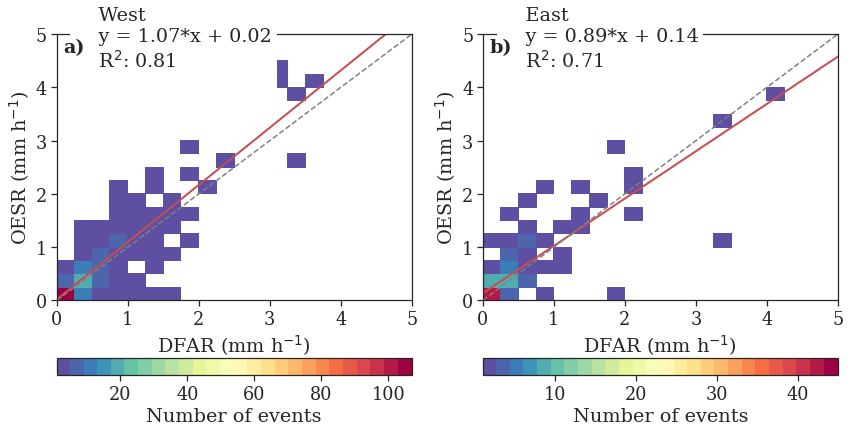
\includegraphics[width=\textwidth,angle=0]{fig8.png}\\
	\caption{Surface snowfall validation of OESR of the hourly snowfall accumulation, with DFAR observations on the x-axis and OESR estimates on the y-axis. The hourly accumulated snowfall amount is separated into westerly snowfall regime in a, and easterly snowfall regime in b. The red line indicates the linear correlation between the DFAR and the OESR surface snowfall accumulation. During westerly snowfall 121 events were counted at the 0.1\,mm\,h$^{-1}$ bin, while during easterly only 45 events were counted at the 0.1\,mm\,h$^{-1}$ bin. The grey dashed lines represent the line of equality where OESR are equal to observations.
	}
	\label{fig:sfc_oesr}
\end{figure}


\begin{figure}
	\noindent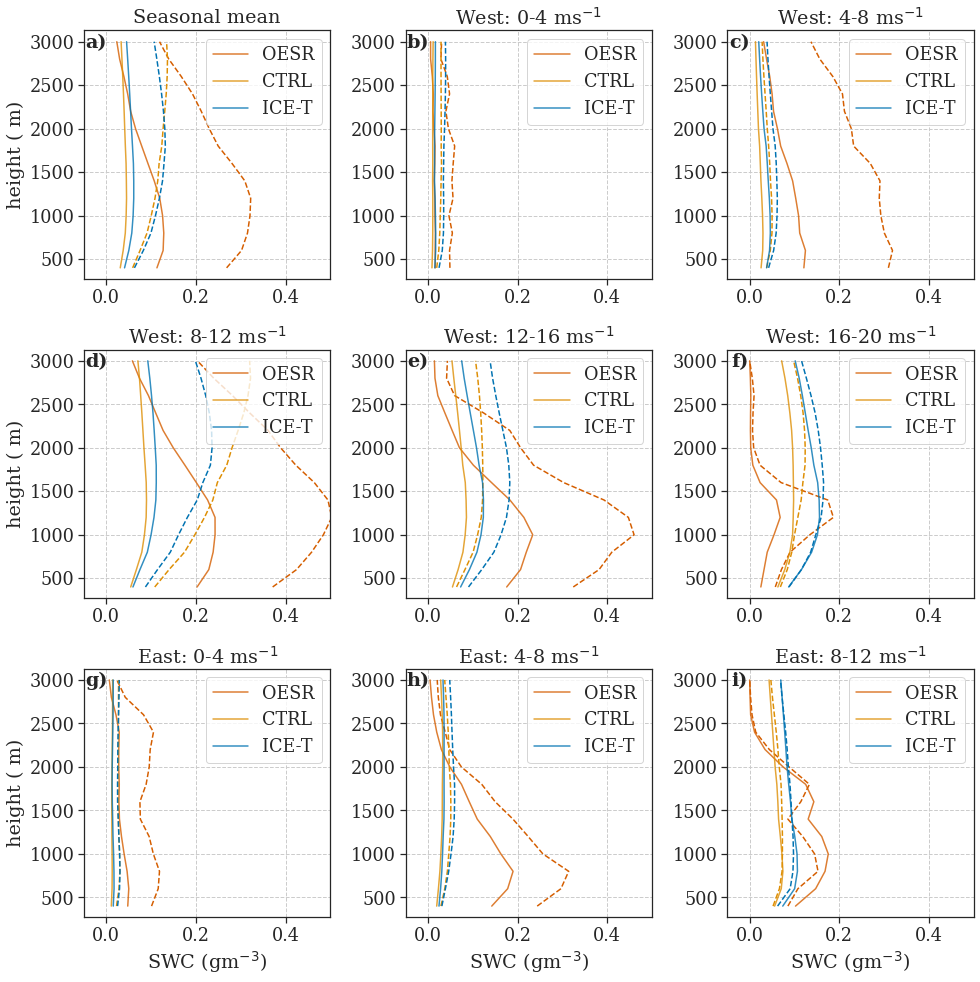
\includegraphics[width=\textwidth,angle=0]{fig9.png}\\
	\caption{Mean (solid) and standard deviation (dashed) of instantaneous SWC separated into west (a-f), east (g-i) snowfall regimes for days fulfilling the analysis requirements during winter 2016-2017. The SWC is sorted into snowfall regimes with the adjusted wind speed correction from the correlation equation in Fig. \ref{fig:WS_correlation}b and c for CTRL and ICE-T, respectively.
	}
	\label{fig:vert_swc}
\end{figure}


\begin{figure}
	\noindent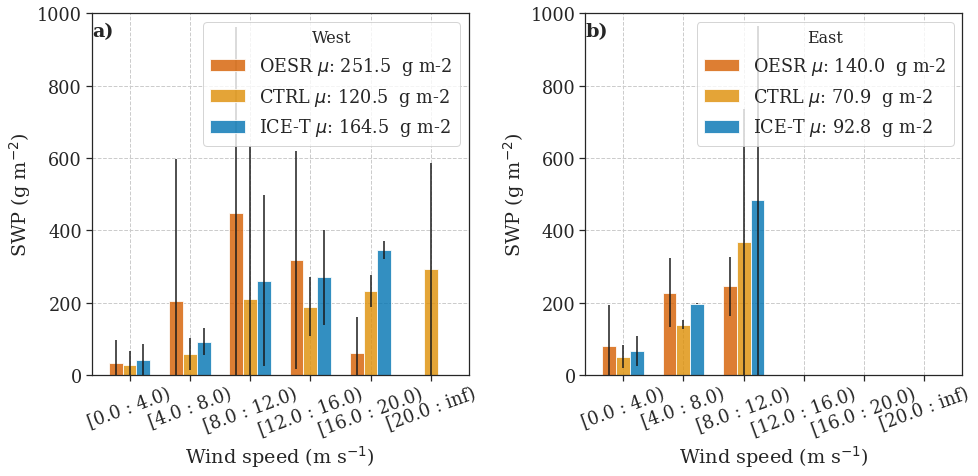
\includegraphics[width=\textwidth,angle=0]{fig10.png}\\
	\caption{Seasonal mean of instantaneous SWP for OESR, CTRL, and ICE-T forecasts separated into westerly and easterly snowfall regimes in a and b, respectively for 27 precipitation days during winter 2016-2017. The separation into wind speed is done with the corrected wind speed bias from Fig. \ref{fig:WS_correlation}b and c for CTRL and ICE-T, respectively. The black line indicates the standard deviation ($\pm \sigma$) in each snowfall wind regime. The mean and standard deviation in each wind speed bin is calculated individually hence the result is dependent on the event hours. The figure labels show the total mean of SWP for over all wind speeds and all precipitation event hours. 
	}
	\label{fig:swp_WS_WD}
\end{figure}


\end{document}